\section{Выбор методологии}

%Жизненный цикл научного ПО краток по сравнению с таковым в
%коммерческой разработке: после проведения измерений, проверки гипотез
%и опубликования результатов (то есть, выполнения цели научной
%программы), продукт как целое быстро утрачивает актуальность ввиду
%развития методов измерений, средств анализа и теоретических моделей.
%При этом отдельные компоненты системы могут
%представлять ценность, и должны допускать повторное
%использование (то есть должны быть в достаточной степени изолированы
%и переносимы). Это обуславливает первое важное требование
%к системе -- модульность.
%
%Модульность предполагает не только декомпозицию программы на
%отдельные семантические узлы, но и предусмотренные конкретным
%техническим средством механизмы замены, дополнения или удаления
%модуля без ущерба для работоспособности системы в целом.
Жизненный цикл научного программного обеспечения обычно короче, чем у коммерческих систем~\cite{lifecycle-lenhardt2014data, Przedzinski2020PhD}: после завершения измерений, проверки гипотез и публикации результатов программный продукт в целом быстро теряет актуальность из-за развития методов измерений, анализа и теоретических моделей~\cite{hep-roadmap-Albrecht2019}. Тем не менее отдельные его компоненты сохраняют ценность и потому должны быть изолированными и переносимыми, что выражается в таком качестве системы как \emph{модульность}. Следует подчеркнуть, что под модульностью понимается не только разбиение программы на функциональные блоки, но и предусмотренная конкретными техническими средствами возможность их замены, дополнения или удаления без ущерба для системы в целом.

%В связи с этим целесообразно обратиться к семейству методологий
%т.н. гибкой разработки программного
%обеспечения (Agile)~\cite{AgileManifesto2001}. В рамках этого семейства,
%каждая методология предлагают построить весь процесс в целом, с расчётом на
%изменчивость отдельных компонент.
Учитывая эту специфику, при проектировании целесообразно опираться на методологии гибкой разработки программного обеспечения (Agile)~\cite{AgileManifesto2001}, которые изначально ориентированы на изменчивость требований и компонентов. Такой подход обеспечивает адаптивность и устойчивость программных систем в условиях эволюции исследовательских задач.

%Хотя монолитность не является неотъемлемым свойством
%таких приложений, в отсутствие усилий по проектированию ПО, часто
%приводит к тому что повторное использование решений становится дороже
%их повторной реализации.

\subsection{Гибкие методологии}

Разработка научного программного обеспечения существенно отличается от
коммерческих практик. Во-первых, здесь отсутствует внешний заказчик
и формализованное техническое задание: постановка задачи формируется
самими исследователями в зависимости от актуальных научных
проблем~\cite{software-for-science-CarverEtAl2016}.
Во-вторых, организационная структура научных групп обычно не
предполагает выделенных менеджеров проектов, и ключевую роль играют
специалисты в предметной области, чьи компетенции в области
разработки программ не обязательно включают беглое понимание
общего контекста, перспектив и стратегии разработки.
В-третьих, часто требуется в сжатые сроки получить конкретный
физический результат (требование высокой доступности решения),
что нередко приводит к компромиссам
в части архитектурной строгости и сопровождаемости кода. Наконец,
значительная доля разработок носит характер рабочих прототипов и
имеет крайне короткий жизненный цикл, ограниченный решением
конкретной вычислительной задачи.

Совокупность этих факторов делает традиционные модели разработки
малоприменимыми и усиливает актуальность гибких методологий,
учитывающих изменчивость требований и обеспечивающих
высокую доступность программного решения. В этом контексте
наибольшую релевантность имеют
три направления из семейства Agile: Domain-Driven Development %(\acrshort{ddd})~\cite{vernon-DDD},
(\acrshort{ddd})~\cite{vernon-DDD},
%(DDD)~\cite{vernon-DDD} \nomenclature{DDD}{Domain-Driven Development\nomrefpage}
обеспечивающее формализацию понятийного аппарата предметной
области; Feature-Driven Development \acrshort{fdd},~\cite{coad1999java-fdd})
%\nomenclature{FDD}{Feature-Driven Development\nomrefpage}
, структурирующее процесс
вокруг реализуемых функций; и Data-Driven Development \cite{Treleaven1982ddd, llopis2009ddd},
ориентированное на построение решений исходя из характера и
динамики обрабатываемых данных.

\begin{comment}
\begin{itemize}
    \item Предметно-ориентированное проектирование
    (<<\emph{Domain Driven Development}>>, \acrshort{ddd})~\cite{vernon-DDD}
    %опирается на глубокое понимание .
    %Согласно этим принципам,
    в рамках которой информационная система проектируется так чтобы
    элементы архитектуры \acrshort{sw} отвечали естественной
    понятийной базе принятой в предметной области, включая специальную
    терминологию, бизнес-логику и т.д.
    \item Разработка управляемая функциями \acrshort{sw} (<<\emph{Feature Driven Development}>>, \acrshort{fdd},~\cite{coad1999java-fdd}) представляет
    собой итеративную методологию, разделяя конечную функциональность
    продукта на отдельные функции. Важно, что на этапе начального
    проектирования, набор функций неполон, не вполне известен и допускает
    изменение уже реализованных спецификаций до окончания жизненного
    цикла \acrshort{sw}.
    \item Проектирование \acrshort{sw} на основе данных (<<\emph{Data Driven Development}>>, первые принципы формулируются в контексте разработки
    процессорных архитектур в
    работе \cite{Treleaven1982ddd}, современное понимание развивается от
    работы \cite{llopis2009ddd})
    подразумевает проектирование и разработку \acrshort{sw} отвечающего
    конкретным количественным критериям.
\end{itemize}
\end{comment}

Нужно подчеркнуть, что в подходе к проектированию на основе данных
под <<данными>> понимают информацию об опыте использования
программного продукта, а не о данных получаемых
при решении научных задач. Тем не менее проектирование на основе
данных находит применение по отношению к высоконагруженным и распределённым
системам, для оптимизации обобщённых
решений в рамках вычислительно-ёмких
процессов~(англ. \emph{High Performance Computing}, \acrshort{hpc})
и вычислений требующих высокой пропускной
способности~(англ. \emph{High Throughput Computing}, \acrshort{htc}).
Несмотря на то что в рамках обобщённой архитектуры приложений для
реконструкции и анализа данных применимость методологии проектирования
на основе данных довольно ограничена, её принципы целесообразно иметь
в виду при проектировании
компонент модульных систем, поскольку на определённом этапе обработка
данных набранных экспериментом осуществляется средствами автоматизированного
пакетного счёта~(\acrshort{htc}), и тогда принципиальными становятся такие черты
архитектуры как стандартизация и обратная совместимость схем и протоколов
(моделей данных, реляционных таблиц, программных интерфейсов),
слабая связность архитектуры и т.д.

\subsection{Гибридный подход}

В рамках разработки архитектуры для реконструкции и анализа данных
физического эксперимента, целесообразно совместить подходы \acrshort{fdd} и \acrshort{ddd},
принимая во внимание следующие положения:

\begin{itemize}
    %\item Сложная понятийная база лежащая в основе разработки
    %отвечает главному принципу \acrshort{fdd} (фокус на предметной области и её
    %модели).
    \item Комплексная предметная область, лежащая в основе
    проектирования, отвечает фундаментальному принципу
    \acrshort{ddd}, в котором ведущая роль отводится предметной области и её
    модели.
    %\item Независимость развития частей модели соответствует
    %ограниченным смысловым и строго согласованным контекстам,
    %декларируемым в \acrshort{fdd}.
    \item Независимая эволюция отдельных частей программного
    решения соотносится с концепцией ограниченных и строго
    определённых контекстов, декларируемых в \acrshort{ddd}.
    \item Эксперитиза профильных специалистов при работе в
    коллаборациях часто требует непосредственной вовлечённости
    в процесс создания и отладки прототипов программ, что
    соответствует коротким циклам инкрементной модели
    развития \acrshort{sw} в \acrshort{fdd}.
    \item На этапе планирования эксперимента возможно формализовать
    и согласовать модель предметной области. Такие черты
    экспериментальной установки, как уровни триггера, периодизация данных,
    каналы реакции, модель трека и кинематика реакций известны
    на проектном этапе. Это позволяет вполне формализовать наборы
    основных сущностей, атрибутов и отношений, что отвечает принципу
    проектирования \acrshort{fdd}.
    \item Высокая доступность продукта (регулярные сборки и
    рабочие релизы) в рамках \acrshort{fdd},
    критически важна для таких этапов жизненного цикла эксперимента,
    как набор данных и проекты развития экспериментальной программы,
    поскольку для них необходимы онлайн-мониторинг работы
    детекторов, моделирование Монте-Карло, а также калибровки
    и экспресс-анализ.
    %отвечает таким важнейшим вариантам
    %использования во время набора данных как онлайн-мониторинг
    %детекторов, моделирование Монте-Карло, получение предварительных
    %численных оценок и калибровок.
\end{itemize}

Следует отметить, что в рамках методологии \acrshort{ddd} под
\emph{контекстом} понимается совокупность ограничений,
обеспечивающих внутреннюю непротиворечивость понятийного аппарата,
в частности согласованное употребление одинаковых терминов.
Так, например, величина интенсивности в общей физике
определяется как энергия, проходящая через единицу площади в единицу
времени, тогда как в физике ускорителей он используется для
обозначения среднего числа частиц, приходящихся на единицу
времени~\cite{Komar1964-accelerators}.

В методологии \acrshort{fdd} понятие контекста определяется менее строго:
под ним обычно подразумевается совокупность допущений и
умолчаний, характерных для конкретной функции или её реализации.

В качестве обобщающего определения, будем понимать далее
под \emph{сценарным контекстом} такой набор вариантов
использования элемента программы, в котором фиксируется
поведение процедур, функций, типов данных и высокоуровневых
сценариев из некоторого набора определяемого предметной области.

Совмещая принципы, изложенные в \cite{coad1999java-fdd, vernon-DDD},
сформулируем следующую последовательность этапов проектирования и
разработки:

\begin{enumerate}
    %\item Выявление предметной области, формирование общей
    %терминологии, классификация (иерархия) вариантов
    %использования. Результатом является перечень основных
    %понятий применяемых в системе.
    \item Анализ предметной области: формирование единого понятийного
    аппарата, выявление ключевых сущностей и обобщённая классификация
    контекстов использования. \\
    \textbf{Ожидаемый результат:} глоссарий основных терминов и концепций,
    применяемых в системе.
    
    %\item Выделение иерархии вариантов использования, задание
    %связанных контекстов (стратегическое моделирование),
    %задающее набор контрактов между контекстами.
    %Результатом является формализованная диаграмма вариантов
    %использования системы.
    \item Структурирование вариантов использования и определение
    связности вариантов внутри контекстов (стратегическое моделирование), задающих
    контрактные границы между ними. \\
    \textbf{Ожидаемый результат:} формализованная диаграмма вариантов
    использования, отражающая взаимодействие контекстов.
    
    %\item Построение доменной модели внутри каждого контекста
    %(основных сущностей, типологии отношений, инвариантов
    %консистентности и правил транзакционной целостности
    %(временные окна, атомарность записи события и т.п.)
    %В качестве результата должны быть диаграммы классов,
    %фиксирующих основные интерфейсы
    %активностей, развёртывания.
    \item Построение детализированной доменной модели внутри каждого
    контекста: определение сущностей, типологии отношений, инвариантов
    консистентности и правил транзакционной целостности (например,
    временные окна фиксации событий, атомарность операций). \\
    \textbf{Ожидаемый результат:} диаграммы классов и интерфейсов,
    фиксирующие основные структурные и поведенческие аспекты системы.
    
    %\item Составление перечня приоритетных элементов системы
    %для реализации.
    \item Определение приоритетных элементов для реализации на ранних
    этапах. \\
    \textbf{Ожидаемый результат:} согласованный перечень функциональных
    компонентов с указанием очередности их внедрения.
\end{enumerate}

Дальнейшая разработка должна производиться в коротких итерационных
циклах сосредоточенных на реализации конкретной функциональности,
необходимой для проведения анализа,
обеспечивая таким образом раннюю проверку проектных решений и их
быструю интеграцию.

%Разработка должна впоследствии производиться в рамках коротких
%циклов разработки отдельных модулей с небольшим сроком отдачи,
%как это предполагается в рамках \acrshort{fdd} со следующими практическими
%рекомендациями:
%\begin{itemize}
%    \item Применение трекера задач и современных СКВ значительно
%    упрощает параллельную разработку
%    \item CI/CD обязательные регулярные сборки, тесты и
%    отчёты о качестве (coverage, performance) обеспечивают высокую
%    доступность и скорость внедрения прототипов решений
%    \item Контракты данных эксплицированные в рамках хорошо
%    определённых схем RPC вроде Protobuf или Avro обеспечивают
%    высокую прозрачность при горизонтальном масштабировании
%    системы.
%\end{itemize}

%В рамках данной работы будем считать понятийный аппарат
%экспериментальной физики во многом известным, и сосредоточимся на
%описании обобщённых контекстов и сценариев использования в них, под которые нужно
%произвести разработку с тем, чтобы выделить конечный набор обобщённых
%решений отвечающий области в целом, предусматривающий
%конкретные точки расширения.
Далее в работе понятийный аппарат экспериментальной физики предполагается преимущественно известным и не требующим детального изложения. Вместе с тем, для устранения возможных разночтений при формулировании ключевых архитектурных ограничений, следует уточнить содержание таких понятий, как <<логический триггер>> и <<объектная модель события>>.

\subsection{Графическая нотация UML}

Для формализации архитектурных решений в данной работе
используется нотация UML 2 (Unified Modeling
Language)~\cite{uml2-std-iso19505-2, uml-2-book-pilone2012umlRU}.
Этот выбор обусловлен тем, что выбранная методология требует
представления программной системы на различных уровнях общности,
описывающих как статические, так и динамические аспекты.
Например, необходимо стратифицировать сценарии взаимодействия
пользователя и системы, необходимо документировать структурные
черты и поведенческие особенности модели. Это существенно выходит
за рамки традиционных блок-схем и диаграмм последовательности,
принятых в отечественных стандартах инженерной
документации (ГОСТ и ЕСПД).

UML является международным стандартом моделирования
программных систем и позволяет единообразно описывать различные
аспекты архитектуры. Несмотря на недостаток формальной
детерминированности этой графической нотации с точки зрения
норм инженерной документации,
использование UML обеспечивает достаточно наглядное представление
систем и отдельных решений посредством
широкого набора выразительных средств, что делает её пригодной
для иллюстрации отдельных аспектов.

\subsection{Виды полиморфизма в точках расширения}
%Инварианты, точки разрешения и виды полиморфизма

В архитектуре программного обеспечения термин \emph{точка расширения}
(англ. \emph{extension point}) относится к идеям проектирования каркасных
систем (англ. \emph{framework}),
в рамках которых различают <<замороженные>> и <<горячие>>
участки кода~\cite{Pree1994-frameworks}. В рамках
классических шаблонов проектирования \cite{gof1994design-patterns},
такие горячие участки
реализуются через паттерны подобные <<фабричному методу>> и служат
средствами обеспечения инверсии управления (внедрение пользовательского
кода). Позднее данный
термин был закреплён в языке UML как обозначение явно заданного места,
в котором поведение варианта использования может быть
расширено\cite{UML-1.5}. На рубеже 2000-х годов концепция точек расширения
получила широкое распространение в т.н. плагин-архитектурах, в
частности в платформе Eclipse~\cite{Eclipse-plugins}, где точка
расширения представляет собой декларативный контракт между ядром
системы и внешним модулем. %Таким образом, точка расширения является
%классическим механизмом задания интерфейсов изменчивости при
%сохранении стабильности архитектурного каркаса.

При выделении точек расширения зачастую необходимо иметь в виду
техническую реализацию: полиморфизм в объектно-ориентированном
программировании определяется как возможность использования единого
интерфейса при множественных реализациях, при этом исполняемая
реализация (конкретное поведение) зависит
от типа объекта \cite{CardelliWegner1985}.

Различают несколько видов полиморфизма (подробная типология полиморфных типов рассматривается в рамках теории т.н. квалифицированных
типов~\cite{krieg1992esop-qualified-types-polymorphism}), однако
в контексте данной работы интересна прежде всего классификация
полиморфизма на \emph{статический} и \emph{динамический} виды.

Динамический полиморфизм
реализуется (в смысле выбора конкретной реализации поведения) во время
выполнения и основан на переопределении виртуальных
методов в иерархиях наследования, с выбором реализации
посредством механизма динамической
диспетчеризации на основе виртуальных таблиц
классов~\cite{Meyer1997, gof1994design-patterns}.
Рисунок \ref{fig:cpp-runtime-polymorphism-example} демонстрирует
пример динамического полиморфизма, в котором виртуальный
метод~\texttt{operation()} класса \texttt{BaseClass} реализуется
в дочерних классах \texttt{DerivedA} и \texttt{DerivedB}.
Языки со строгой типизацией (C++) опираются в основном на динамический
полиморфизм и предоставляют специализированную лексику.

\begin{figure}
    \centering
    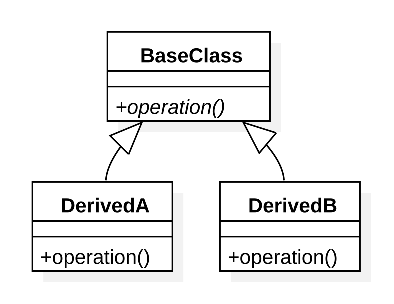
\includegraphics[width=0.35\linewidth]{images/illustrative/runtime polymorphism.eps}
    \caption{Пример реализации динамического полиморфизма виртуального метода на диаграмме классов}
    \label{fig:cpp-runtime-polymorphism-example}
\end{figure}

Важно заметить, что в C++ не включены специальные лексические средства для
описания интерфейсов, как это сделано в таких языках как Java
или C\#. В C++ интерфейс, как элемент неявно включён в виртуальный
класс. В то же время, в тех случаях, когда по каким-то причинам,
интерфейс всё же должен быть обозначен в коде программ сам по себе,
прибегают к идиоматическому представлению посредством объявления абстрактного класса
(или структуры) не содержащего атрибуты, с одними чисто-абстрактными
методами. В этом случае, структура типов выглядит подобно примеру
изображённому на рисунке~\ref{fig:cpp-runtime-polymorphism-example-w-iface},
где интерфейс \texttt{BaseClass} вынесен в отдельный тип
данных~\texttt{BaseClassIFace} обобщающий класс~\texttt{BaseClass},
наследники которого уже и реализуют интерфейс.

\begin{figure}
    \centering
    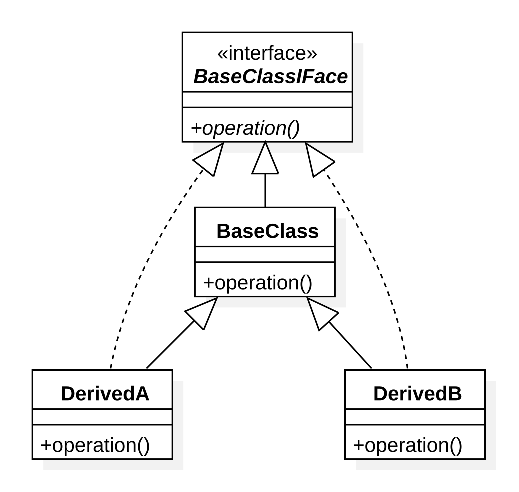
\includegraphics[width=0.5\linewidth]{images/illustrative/runtime polymorphism w iface.eps}
    \caption{Пример реализации динамического полиморфизма в C++ с выделенным интерфейсом на диаграмме классов}
    \label{fig:cpp-runtime-polymorphism-example-w-iface}
\end{figure}

Статический полиморфизм
разрешается на этапе компиляции, обычно через перегрузку функций
и операторов, а также шаблоны \cite{Stroustrup2013}.
Статический полиморфизм в C++ широко используется для достижения
настраиваемого поведения на этапе компиляции без накладных
расходов динамической диспетчеризации. Он реализуется
посредством т.н. traits-типов (в ряде источников -- \emph{свойства},
\emph{шаблоны свойств}), частичной или полной специализации
шаблонов, часто с применением идиомы
\acrshort{sfinae} (англ. \emph{Substitution failure Is not an error},~\cite{Vandevoorde2002-cpp-templates}) -- то есть
механизмом, позволяющим исключать неподходящие
шаблонные инстанцирования при разрешении перегрузок, реализуя,
таким образом систему \emph{классов типов}, подобную той что применяется в
некоторых функциональных языках (Scala, Haskell). Кроме
того, статический полиморфизм может быть достигнут с
помощью идиомы \acrshort{crtp}~(англ. \emph{curiously recurring template pattern},~\cite{Abrahams2005-cpp-metaprogramming}),
при котором классы наследуют шаблон, параметром которого является
сам класс-наследник, что обеспечивает разрешение виртуальной
функциональности на этапе компиляции.

Пример статического полиморфизма с использованием traits-типа
изображён на рисунке \ref{fig:cpp-static-polymorphism-example}.
В качестве полиморфной сущности рассмотрен
класс~\texttt{Subject} параметризуемый типом~\texttt{T}.
Класс~\texttt{Subject} содержит обобщённую программу, в которой
определения типов, вызов конкретных процедур или использование
определённых значений делегируется некоторому шаблонному
типу~\texttt{Traits}, параметризуемому типом~\texttt{T}, в общем
случае не обязательно определённому.
В этом случае, возможно определять полные или частичные (в т.ч.
с использованием \acrshort{sfinae}) специализации типа~\texttt{Traits<T>}
во внешних модулях программ, таким образом дополняя и обогащая
реализации обобщённых алгоритмов в~\texttt{Subject<T>}
соответствующими расширениями. В приведённом примере
инстанцирование шаблона~\texttt{Subject<float>} выводит
конкретную реализацию~\texttt{Subject} на основе информации
предоставленной~\texttt{Traits<float>}.

\begin{figure}
    \centering
    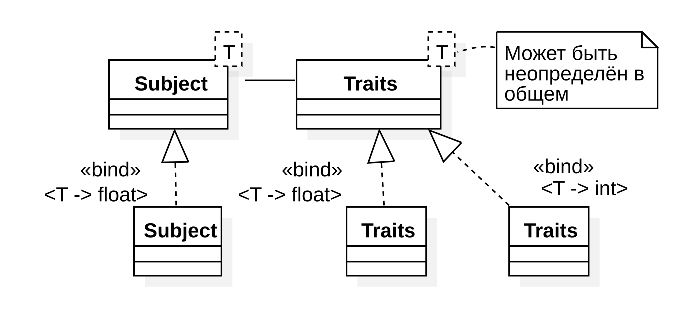
\includegraphics[width=0.7\linewidth]{images/illustrative/static-polymorphism-example.eps}
    \caption{Пример статического полиморфизма на основе шаблона свойств}
    \label{fig:cpp-static-polymorphism-example}
\end{figure}

%Хотя по очевидным причинам, статический полиморфизм эффективен
%с вычислительной точки зрения, с точки зрения практической разработки,
%важно, что реализация статического полиморфизма в C++ посредством
%идиом CRTP и SFINAE представляет собой достаточно сложные для
%сопровождения и отладки лексические конструкции. 
Хотя статический полиморфизм обладает очевидными преимуществами
с вычислительной точки зрения, его практическое использование в C++
сопряжено с определёнными трудностями. Реализация посредством идиом
\acrshort{crtp} и \acrshort{sfinae} приводит к возникновению сложных для сопровождения
и отладки лексических конструкций (грамматика
языка шаблонов исторически вводились в C++ поверх существующего
стандарта языка, и не предусматривает соответствующей
функциональности в виде явных лексических конструкций).
Кроме того, статический полиморфизм характеризуется высокой
инфраструктурной инвазивностью.
По этим причинам,
решение о предоставлении публичным \acrshort{api} точки расширения
реализуемой посредством статического полиморфизма, должно приниматься
в рамках глобальной архитектуры приложений.
%, что делает его использование
%в качестве механизма расширения публичного
%\acrshort{API} оправданным лишь в случае, если такое решение согласовано
%с общей архитектурой системы.


%Основное внимание в последующем изложении уделено описанию обобщённых контекстов и типовых сценариев использования, которые служат основой для разработки
%соответствующих технических решений, с указанием соответствующих
%принципиальных ограничений. Целью главы является выделение конечного
%набора обобщённых решений, охватывающих потребности рассматриваемой
%области в целом и формализующих её типовые задачи, при этом
%предусматривается определение конкретных точек расширения,
%позволяющих адаптировать эти решения к специфическим условиям отдельных
%экспериментов, подсистем и этапов исследований.

\begin{comment}
Дальнейшее изложение сосредоточено на описании обобщённых контекстов и типовых сценариев использования, которые образуют основу для разработки соответствующих технических решений с фиксацией их принципиальных ограничений. Целью главы является выделение конечного набора обобщённых решений (\emph{инвариантов} системы),
охватывающих совокупность потребностей рассматриваемой области и
формализующих её характерные задачи. При этом предусматривается
определение конкретных \emph{точек расширения}, обеспечивающих адаптацию
указанных решений к специфическим условиям отдельных экспериментов,
подсистем и этапов исследований.
\end{comment}